\documentclass{article}

\usepackage[a4paper, total={15cm, 24.5cm}]{geometry}
\usepackage{float}
\usepackage{graphicx}
\usepackage{amsmath}
\usepackage{caption}
\usepackage{subcaption}

\usepackage[dvipsnames]{xcolor}
\usepackage{listings}
\lstloadlanguages{Ruby}
\lstset{
	basicstyle=\ttfamily\color{black},
	commentstyle = \ttfamily\color{green},
	keywordstyle=\ttfamily\color{blue},
	stringstyle=\color{orange}}

\title{Advanced Algorithms and Parallel Programming}
\author{Elia Ravella}
\begin{document}
	\begin{titlepage}
		\maketitle
	\end{titlepage}
	
	\tableofcontents
	\clearpage

	\part{Advanced Algorithms}
	\section{Algorithms Recall}
		An algorithm is a well defined computational procedure that takes some value as input and produces some value as output after a finite sumber of steps.
		
		\paragraph{Algorithm Performance - Complexity}
			A straightforward performance index for an algorithm is his running time. Obviously, the running time depends on the size of the input, so making the performance index parametric wrt the input size is the best way to compare algorithms. Generally, we look for upper bounds of running time, as a guarantee; but three main analysis can be carried out:
			\begin{itemize}
				\item worst case scenario (big $O$ notation): maximum time of the algorithm for an input of fixed size
				\item average case scenario ($\Theta$ notation): expected time for a fixed size input. To comeplete an analysis like this one, we need assumption on the distribution of the input
				\item best case scenario ($\Omega$ notation): analize the \textit{minimum time required to terminate} with the best possible combination of input. It's useful because provides a lower bound of performance for an algorithm (we "can't do better" with that algorithm)
			\end{itemize}
			When we compare complexity curves, we must not forget the fact that those are dependent from the input instance size. For sufficently large inputs, then a $n^2$ complexity always beats an $n^3$, but it's not so when instances are small enough. Use complexity to help structure the design phase, not as the one and only performance index to use.

			\subparagraph{The Master Method}
				To solve recurrencies (analysis of complexity for algorithms expressed as mere time functions of the input) of the form
				\begin{equation}
					T(n)\, =\, aT(\frac{n}{b})\, +\, f(n)
				\end{equation}
				where $a \geq 1$, $b > 1$ and f is asymptotically positive, we can use the \textit{master method}, that gives use the complexity for three common cases, basing itself on the $f(n)$ function:
				\begin{itemize}
					\item $f(n) = O(n^{\log_ba\, -\, \epsilon})$ for some $\epsilon > 0$. The total algorithm complexity then is
						\begin{equation}
							T(n) = \Theta(n^{\log_ba})
						\end{equation}
					\item $f(n) = \Theta(n^{\log_ba} \log_e^kn)$ for some $k \geq 0$. The total algorithm complexity then is
						\begin{equation}
							T(n) = \Theta(n^{\log_ba} \log_e^{k+1}n)
						\end{equation}
					\item $f(n) = \Theta(n^{\log_ba\, +\, \epsilon})$ for some $\epsilon > 0$. The total algorithm complexity then is
						\begin{equation}
							T(n) = \Theta(f(n))
						\end{equation}
				\end{itemize}

	\section{Design Paradigms for Algorithms}
		\subsection{Divide and Conquer}
			Super classic algorithmic approach to problem solving:
			\begin{enumerate}
				\item Divide the problem into simple subproblems
				\item Solve the subproblems, if needed recursively divideng them further
				\item Combine the results
			\end{enumerate}

			\paragraph{Merge Sort}
				DeC applied to sorting results in the famous merge sort algorithm:
				\begin{enumerate}
					\item Split the array
					\item Sort the two subarrays
					\item Linear time merge
				\end{enumerate}
				resulting in a total complexity of $T(n) = 2T(\frac{n}{2}) + \Theta(n)$ that can be easily worked out with the master theorem: it falls in the second case with k = 0. This leaves us with a total complexity of $\Theta(n\, \log(n)$.

			\paragraph{Binary Search}
				DeC applied to searching an element in a \underline{sorted} array
				\begin{enumerate}
					\item Check middle element
					\item Recursively search a single subarray
					\item Find element
				\end{enumerate}
				total complexity: $T(n) = T(\frac{n}{2} + \Theta(1)$. Again, through the Master Method, we obtain a complexity of $T(n) = \Theta(\log(n))$

			\paragraph{Number Power}
				Computing $a^n$ in underlinear complexity: with divide and conquer is possible. Just apply
				\begin{equation}
					a^n = 
					\begin{cases}
						a^{\frac{n}{2}}\cdot a^{\frac{n}{2}} \text{ when the exponent is even}\\
						a^{\frac{n-1}{2}}\cdot a^{\frac{n-1}{2}} \cdot a \text{ when the exponent is odd}
					\end{cases}
				\end{equation}
				This algorithm has the same complexity of the binary search one: $T(n) = \Theta(n)$

			\paragraph{Matrix Multiplication}
				Row per coloumn multiplication of two matrixes, standard algorithm executes in $\Theta(n^3)$, it mimics the "by hand" procedure. DeC approach: consider each matrix as a $2\, \times\, 2$ matrix of submatrixes that are "half the lenght", and then recursively go down to the single elements. in the end, add all.\\
				Resulting complexity:
				\begin{equation}
					T(n) = \underbrace{8T(\frac{n}{2})}_{\text{the 8 resulting submatrixes}} + \underbrace{\Theta(n^2)}_{\text{adding the matrixes together}}
				\end{equation}
				With the master method, we still obtain a complexity of $\Theta(n^3)$ (case 1) so no improvement. The winning idea here is to reduce the number of multiplications needed to find the result of the reduced problem, from 8 to 7, using the Strassen's algorithm. This then changes the first term in the complexity description to $T(n) = 7T(\frac{n}{2}) + \Theta(n^2)$. We still fall in the first case of the Master Method, but this time the difference is in the exponent, reduced from 3 to 2,81. The improvement here is noticeable in not-so-small instances of the problem, of course, and become way more significant when the instances dimension grows.

	\section{Randomized Algorithms}
		Randomized algorithms exploits some probabilistic features of the inputs in order to run "at best on the average case". We call a randomized algorithm an algorithm that depends not only on the input it's given, but also on a random number generated inside the algorithm.\\
		To actually evaluate the performances of the algorithm we make use of \textit{indicator random variables} that are simple binary variables that indicates wheter something is happened or not.

		\subsection{Monte Carlo Algorithms}
			Monte Carlo algorithms are randomized algorithms that \textit{can return a wrong result}, but with little probability. In the case this probability is non null, the problem is said to have a \textit{two sided error}.
	
			\subsubsection{Las Vegas Algorithms}
				Las Vegas algorithms are randomized algorithms that (differently from Monte Carlo ones) \textit{always return correct results}, but they directly depends on some random  choices; this implies that the running time can vary even with identical input, thus rendering the \textit{average running time} very difficult to compute.

			\subsubsection{Karger's min-cut algorithm}
				Minimum cut problem: to find the cut (on a connected undirected weighted graph) with the \textit{minimum possible capacity}. The general algorithm computes $n - 1$ times the so called "st-cut problem", that only considers the "weight flow" between two fixed nodes. Karger's approach is based on randomization and contractions\footnote{make two nodes coincidental in a graph, "collapse"}: by contracting together nodes we will eventually find a cut of the graph, that will be represented by the arcs that go through the "central most contracted node".\\
				So the Karger algorithm translates to:
				\begin{enumerate}
					\item pick a random edge
					\item contract it (doing so, remove self-loops)
					\item repeat 1 and 2 until the graph has only two nodes
					\item check the obtained cut
					\item repeat in case
				\end{enumerate}
				The average complexity is far less that the linear programming formulation of the problem. Moreover, statistically speaking and given enough runs, the Karger's algorithm finds the solution far before the "traditional" linear programming algorithm, that runs in $O(n \cdot m \cdot \log (\frac{n^2}{m}))$ where \emph{n} and \emph{m} represent nodes and edges number, respectively.\\
				An improved version of this algorithm was provided by Karger himself, after the observation that is very unlikely to pick a min cut edge \textit{at the beginning} of the algorithm wrt the end of the procedure. The thing that changes here is the last step of the algorithm: instead of restarting from the beginning (so from the complete graph) it restarts from an \textit{intermediate graph} with a reduced number of nodes and then compares the two obtained results. This improvement is huge: it reduces the running time to $n^2 \cdot \log(n)$, with an error probability that's polynomial.

			\subsubsection{Randomized Quicksort}
				Classic quicksort is an $O(n \log (n))$ in place sorting algorithm, using the divide and conquer approach. The algorithm can be seen as an "in place merge sort": it divides the algorithm around a \textbf{pivot} element and recusively sort the two portions of array.\\
				The random formulation introduces randomness in the pivot selection, in particular in the selection of the indexes that produces the pivot. This ensures that the running time is \textit{indipendent} of the input order. We end up with an average complexity of $n \log (n)$.
				\begin{lstlisting}[language=Ruby]
# randomized adjustement to quicksort algorithm, where the pivot is 
# randomly chosen each time
def rand_partition(arr, bottom, top)
  pivot = Random.new.rand(bottom..top)

  swap = arr[pivot]
  arr[pivot] = arr[top]
  arr[top] = swap
  return partition(arr, bottom, top)
end

# partitioning and swapping subroutine
# this just moves the lower values to the left 
# and the higher to the rights
def partition(arr, bottom, top)
  last = arr[top]
  first = bottom - 1

  for current in bottom..(top - 1)
    if arr[current] <= last
      first = first + 1

      # swap elements
      swap = arr[current]
      arr[current] = arr[first]
      arr[first] = swap
    end
  end

  # swap the highest left value with the right value
  # from the pivot point of view
  swap2 = arr[first + 1]
  arr[first + 1] = arr[top]
  arr[top] = swap2

  return (first + 1)
end

# simply divide
def quicksort(arr, bottom, top)
  if bottom < top
    pivot = rand_partition(arr, bottom, top)
    quicksort(arr, bottom, pivot - 1)
    quicksort(arr, pivot + 1, top)
  end
end              
				\end{lstlisting}
				Complexity analysis of quicksort and randomized quicksort: we can see how the PARTITION subprocedure, when it's not randomized, can yield to an optimal case, where the array is split in half, and a worst case, where the array is split in a $n-1$ long subarray and another of length zero. So the randomized approach ensures that the recursion tree of this procedure is always $\Theta(\log(n))$ and having $O(n)$ work done at each level we end up with $O(n \cdot \log(n))$.\\
				We should focus on the PARTITION subprocedure because it's the core of the complexity of the entire algorithm, and because it has two interesting properties:
				\begin{enumerate}
					\item the time spent in there dominates the complexity of the algorithm
					\item it's called \textit{at most} \emph{n} times					
				\end{enumerate}
				the call itself is a $O(1)$ operation plus the complexity induced by the \verb|for| loop that swaps the elements in the array. So, the total complexity of the algorithm \textit{heavily depends} on the number that the instruction \verb|if arr[current] <= last| is executed. Our aim is this, to compute \emph{X} the number of comparisons performed across all calls to PARTITION. So the total complexity of the algorithm is $O(n + X)$. $X_{ij}$ is so the indicator binary variable for "element \emph{i} is compared with element \emph{j}". Obviously, $X = \Sigma_{i = 1}^{n-1} \Sigma_{j = 1}^{n} X_{ij}$. If we apply the expexted value operator to this formula we are left with the probability that element \emph{i} is compared with element \emph{j}.\\
				This is:
				\begin{align*}
					Pr\{z_i \text{ is compared to } z_j\} = Pr\{z_i \text{ or } z_j \text{ are chosen as pivot }\} = \\
					= \frac{1}{\text{number of elements in subarray}} \times 2 = \\
					= \frac{2}{i - j + 1}
				\end{align*}
				Substituting this equation in $E[X] = E[\Sigma_{i = 1}^{n-1} \Sigma_{j = 1}^{n} X_{ij}]$ we obtain
				\begin{align*}
					E[X] = \sum_{i = 1}^n \sum_{j = 1}^{n - 1} \frac{2}{i - j + 1} \\
					< \sum_{i = 1}^n \sum_{j = 1}^{n - 1} \frac{2}{i - j} \\
					= \sum_{i = 1}^{n - 1} O(\log(n)) = O(n \cdot \log(n)) \text{ armonic series}
				\end{align*}
						
			\subsubsection{Randomized Selection - Order Statistics}
				The algorithm can be described as "find the \emph{i}-th smallest/greatest number of a collection", so the element with rank \emph{i}. The naive idea is: sort the collection ($\Theta(n \cdot \log(n))$) then take the \emph{i}-th element ($\Theta(1)$). Total complexity: $\Theta(n \cdot \log(n))$.\\
				There's an algorithm, derived from quicksort\footnote{it even uses the same RANDOMIZED-PARTITION function}, with expected running time in $\Theta(n)$ to find the \emph{i}-th element, which has $\Theta(n^2)$ as worst case complexity.\\
				The algorithm is quite simple: it uses the RANDOMIZED-PARTITION function of the quicksort algorithm in order to partition the array around a pivot element (choosen at random): after that, all the smaller elemets will be on the left and the greater on the right. Then, it checks if the \textit{order statistic} is equal to the number of elements in the "lesser" subarray, adding 1 to this value to keep track of the pivot element itself. If they're equal, we've found our element. If not, we resort to check a single subarray of the two:
				\begin{itemize}
					\item the greaters one if the order statistic is greater than the number of elements in the first subarray
					\item the smallers if not
				\end{itemize}
				\begin{lstlisting}[language=Ruby]
def select_ith(arr, head, tail, order_statistic)                                                                                                                       
  return arr[head] if head == tail
  
  # so now we've partitioned the array
  pivot_index = rand_partition(arr, head, tail)

  # temptative represents the k-th index of the array
  temptative = pivot_index - head + 1 

  if temptative == order_statistic
    return arr[pivot_index]
  elsif order_statistic < temptative
    return select_ith(arr, head, pivot_index - 1, order_statistic)
  else
    return select_ith(
      arr, 
      pivot_index + 1, 
      tail, 
      order_statistic - temptative
    )
  end
end
				\end{lstlisting}
				The complexity is given by the recurrence
				\begin{equation}
					T(n) \leq \sum_{k = 1}^n (X_k \cdot (T(\max(k - 1, n - k))) + O(n))
				\end{equation}
				Where
				\begin{itemize}
					\item $X_k$ is a binary variable that is 1 for the \emph{k}th partition when it produces a \emph{k} elements split. This variable is here to help with the expexted value analysis, because it has $E[X_k] = \frac{1}{n}$.
					\item $T(\max(k - 1, n - k))$ is the \textit{pessimistic assumption} of this recursion: in order to calculate an upper bound, we hypotize that the element we're looking for is always in the bigger subarray
				\end{itemize}
				\begin{align*}
					\sum_{k = 1}^n (X_k \cdot (T(\max(k - 1, n - k))) + O(n)) = \sum_{k = 1}^n (X_k \cdot (T(\max(k - 1, n - k)))) + O(n) \\
					\Rightarrow E[T(n)] = \sum_{k = 1}^n (\frac{1}{n} \cdot E[(T(\max(k - 1, n - k)))) + O(n) 
				\end{align*}
				The problem here is that $\max$ function in the center of the recurrence. But, we can analyze the two subproblems to get rid of it. We knwo that that function will return
				\begin{equation}
					\max(k - 1, n - k) =
					\begin{cases}
						k - 1 \text{ when } k > \lceil \frac{n}{2} \rceil \\
						n - k \text{ when } k \leq \lceil \frac{n}{2} \rceil
					\end{cases}
				\end{equation}
				if \emph{n} is even, being \emph{k} spanning from 1 to \emph{n}, we have that the first $\frac{n}{2}$ terms appears exactly twice, so $\max(k - 1, n - k) = 2k$. If not, we simply have an "extra term" that is $\lfloor \frac{n}{2} \rfloor$.\\
				We end up with
				\begin{equation}
					E[T(n)] = \frac{2}{n} \sum_{k = \lfloor \frac{n}{2} \rfloor}^{n-1}(T(k)) + O(n)
				\end{equation}
				where $T(k) = O(n)$ can be proven by substitution.

			\subsubsection{Primality Test}		
				For "primality test" is intended the boolean procedure to verify if a number is actually a prime number (so is divisible only for itself and 1). The super naive approach is to check if the number is 2, check then parity, then cycle through 3 and $\frac{\sqrt{n}}{2}$ to find a evenly divisor of the considered number.
				\begin{lstlisting}[language=Ruby]
def is_prime(n) 
  return false unless n.is_a? Integer
  if n%2 == 0                                                                                                    
    return false                                                                                                 
  else                                                                                                            
    (3..(Integer.sqrt(n)/2).floor()).each {                                                                       
      |d|                                                                                                        
      return false if n%(2*d + 1) == 0                                                                           
    }                                                                                                            
  end                                                                                                            
  true                                                                                                            
end   
				\end{lstlisting}
				This algorithm has a $\Theta(\sqrt{n})$ complexity.\\
				The randomized version is a one-sided error, false biased Monte Carlo algorithm: the result is always correct if negative, and can be wrong (with a little probability) if it's positive. This exploits the Fermat's Theorem: "each odd prime numbers divides $2^{p - 1} - 1$". So a polynomial approach can be: calculate $z = 2^{n - 1} \,mod\, n$ and check if it's 1: then the number it's possibly prime, otherwise surely isn't (it's composite). This test is also called pseudoprimality test, because numbers that satisfies such property are called \textit{base-a pseudoprimes}, where \emph{a} is the base of the power(2, in our case). The probability to find a pseudoprime that's not prime in a $\beta$-bit encoded number tends to zero when $\beta \,\rightarrow\, \infty$. In a 1024-bit encoded number, the probability of random picking a base-2 pseudoprime that is not prime are less that 1 in $10^{41}$: this makes this version of the algorithm useful (and insanely fast) for most of the usual applications.
				\begin{lstlisting}[language=Ruby]
def is_pseudoprime(n)
  return false unless n.is_a? Integer
  return (2**(n - 1) % n == 1)                                                                                    
end
				\end{lstlisting}
				We actually cannot get rid of the small error margin of this algorithm, due to Carmicheal numbers\footnote{I don't want to go down this algebraic-arithmetic rabbit hole, ok?}.

				\paragraph{Miller Rabin Las Vegas Version}
					Actually, a Las Vegas version of the primality test does exist, and it's a modification of the previous algorithm that introduces randomization. The two main changes are:
					\begin{itemize}
						\item base \emph{a} is not fixed, but chosen at random. Also, in an iteration several values are tried
						\item It performs an additional "nontrivial square root" check, that if succeeds signals a composite number
					\end{itemize}
					The nontrivial square root check is fairly simple, as the definition of a nontrivial square root is: \emph{a} is a nontrivial square root of $1 \mod n$ if $a^2 \mod n = 1 \wedge a \neq 1 \wedge a \neq n - 1$. Do not be scared! That only means that \emph{a} is the square root of a number that's \textbf{\underline{modulo equivalent}} to $1 \mod n$. We will use this to prove that a number is not composite. Here's some Ruby code that implements that:
					\begin{lstlisting}[language=Ruby]
is_probably_prime = false

def power(base, iter, number)
  # recursive computation of the power of the number
  # in order to find a nontrivial square root

  return 1 if iter == 0
  
  # computation of the factors
  x = power(base, iter/2, number)
  result = x**2 % number

  # nontrivial square root check
  if (result == 1 and x != 1 and x != number - 1)
    is_probably_prime = false 
  
  # result computation: notice how variable "result" is recomputed
  result = (base * result) % number if iter % 2 == 1

  return result
end

def MR_primality_test(n)
  base = Random.new.rand(2..(n - 1))

  res = power(base, n - 1, n)
  
  is_probably_prime = true

  return false if res != 1 or !is_probably_prime
  true
end
					\end{lstlisting}

	
	\section{Sorting Lower Bounds and Linear Sorting Algorithms}
		\subsection{Comparison Sorts and Lower Bounds}
			Comparison sort algorithms are algorithms that swaps elements of an ordered collection comparing them one another, to eventually order it. We could see this as a continuous exploration of the "permutations space" of the original collection, until we find the right one. Being a systematic procedure, sorting can be represented as a \textbf{decision tree traverse} procedure. This procedure is useful to calculate the theoretical lower bound in complexity for the comparison sort algorithms.\\
			If we build a decision tree where every node corresponds to a comparison of our sorting algorithm, and every leaf a permutation of the initial collection, we end up with a representation of all the decisions/comparison that the algorithm should face until it can reach the solution, and the height of that tree would be the worst case running time (each path from the root to a leaf represents an algorithm run). Since the tree must contain more than $n!$ leaves, we have that our decision tree\footnote{that's a BINARY tree} has $2^h \geq n!$ leaves, where \emph{h} is the height of the tree. Concisely, a lower bound in the height of the tree corresponds to a lower bound in the number of comparinsons needed to sort an array. This leads to the equality
			\begin{equation}
				h = \Omega(n \cdot \log (n))
			\end{equation}
			Coming from
			\begin{equation}
				n! \leq 2^{height} \,\Rightarrow\, height \geq \log(n!) \,\Rightarrow\, \underbrace{height \geq \log((\frac{n}{e})^n)}_{Stirling's formula} \,\Rightarrow\, \Omega(n \cdot \log(n))
			\end{equation}

		\subsection{Linear Time Sorting}
			The counting sort and the radix sort are two algorithms that sort collections in linear time. How is this possible? They do not rely on \textit{comparisons} and they make strong assumptions on input types.

			\paragraph{Counting Sort}
				Counting sort is an \textit{array}-sorting algorithm that deals with \textit{small positive integer numbers}. "Small" in the sense that there should be an upper bound to them. The algorithm uses an auxiliary array where it accumulate the occurences of every element of the original one (populating the cells of the aux. array by using the original integers as indexes). When the first traversal is completed, we start from the bottom of the sorting array and we confront the value of the element with the value in the aux element associated to it (so that uses that value as index). We put that value at the index pointed, and we decrease the counter (in the second array). At the end of the second traversal, we've sorted the array. $O(n + k)$ complexity, where \emph{k} is the highest integer number in the array.\\
				Possible ruby implementation (pay attention to the 4-loops construction of the algorithm):
				\begin{lstlisting}[language=Ruby]
def counting_sort(arr)
  auxiliary = Array.new (arr.max + 1)
  output = Array.new arr.length

  # set structures to zero
  auxiliary.map! { |x| x = 0}
  output.map! { |x| x = 0 }

  # record positions
  arr.each do |i|
    auxiliary[i] += 1
  end

  # accumulate
  i = 0
  while i < auxiliary.length - 1
    auxiliary[i + 1] += auxiliary[i]
    i += 1
  end

  # reconstruct array
  i = arr.length - 1
  while i >= 0
    output[
      auxiliary[
        arr[i]
      ]
    ] = arr[i]
    auxiliary[arr[i]] -= 1
    i -= 1
  end

  return output
end
				\end{lstlisting}

			\paragraph{Radix Sort}
				Radix sort exploits digit-by-digit sort, using counting sort to sort the digits. The original implementation sorts starting from the most significative digit, but the latter on (the right one) sorts starting from the least significant digit. The application is quite straightforward: counting sort is applied \textit{to the whole number} but considering \textit{only the least significant digit not yet analyzed} for the sortings. The stability of the counting sort (property to preserve relative order between equal numbers) ensures that the final array is sorted.


	\section{Advanced Data Structures}
		\subsection{Disjoint Sets}
			Disjoints set are a \textit{collection of collections} where all the subcollections are \textit{disjoint} (no element is in more than one set) and each subset is represented from an element of that set. Usually the choice of the representative element is not crucial to the functioning of the structure.

			\subsubsection{Operations on a Disjoint Set}
				Disjoint sets must be capable of performing these operations:
				\begin{enumerate}
					\item \verb|MAKE-SET(x)| the basic wrapper, that puts "x" into a set. Naturally, "x" should not be in another set.
					\item \verb|UNION(x, y)| performs the set union of the two sets that constains \emph{x} and \emph{y}, $S_x$ and $S_y$. This operation removes $S_x$ and $S_y$ from the structure (their elements would be duplicated) and merges the two sets into a new one. A representative is either chosen a priori or recomputed.
					\item \verb|FIND-SET(x)| returns a reference to $S_x$.
				\end{enumerate}

			\subsubsection{Implementation: Linked List}
				A super easy way to implement disjoint sets is through linked lists, where each list represents a subset. The structure for each set holds a pointer to the head and one to the tail of the list, to facilitate operations (as \verb|UNION|).
				\begin{figure}[H]
					\centering
					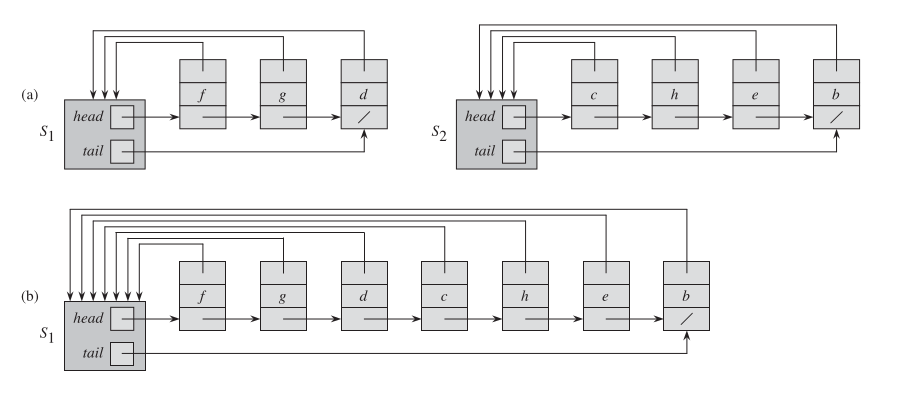
\includegraphics[width = \textwidth]{images/union.png}
					\caption{A union performed on a disjoint set implemented through linked lists}
				\end{figure}
				The union operation takes $\Theta(n^2)$. Can we do better?

			\subsubsection{Implementation: Forest}
				Instead of using linked lists to represent the sets, use instead a tree (also not binary) that has the set-representative in the root element. A disjoint set will then be a forest, where each tree is a set. This time the \verb|FIND-SET| operation takes $O(\log(\text{element of the subset}))$ and the \verb|UNION| is straightforward: just "append" a tree to the other's root, $O(1)$
				\begin{figure}[H]
					\centering
					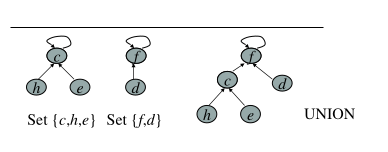
\includegraphics[width = \textwidth]{images/forestUnion.png}
				\end{figure}
				I've spent a week on this DisjointSet class in Ruby, using no optimizations. So, here it is:
				\begin{lstlisting}[language=Ruby]
class DisjointSet
  attr_accessor :sets # forest for sets

  def initialize
    @sets = Array.new
  end

  def make_set(element)
    if (sets.filter { |i| i.has(element)}).length == 0
      @sets.push(Tree.new(element))
    end
  end

  def find_set(element)
    i = 0
    while i < sets.length
      return sets[i]  if sets[i].has(element)
      i = i + 1
    end
    return nil
  end

  def set_insert(representative, element)
    i = 0
    while i < sets.length
      if sets[i].root.value == representative
         @sets[i].insert(element)
         break
      end
      i = i + 1
    end
  end

  # unite the two sets corresponding to the elemenents
  def union(element1, element2)
    set1 = find_set(element1)
    set2 = find_set(element2)

    return nil if set1.nil? or set2.nil?

    set1.insert_node(set2)

    sets.delete(set2)
  end

  def show
    for i in sets
      print "->"
      i.show
    end
  end
end
				\end{lstlisting}
				This implementation can be furtherly optimized, using ranking and path compression:
				\begin{itemize}
					\item Union by \underline{ranking}: when uniting trees, always look at the rank of the tree itself (that's the height of the tree) and attach the "smaller" to the "greater"
					\item \underline{Path compression}: contextually a \verb|FIND-SET| operation, make all the subtrees' root point directly to the representative (reducing total tree height)
				\end{itemize}
				applying both these optimizations (that are merely \textit{heuristics}) we can achieve a worst case running time of $O(m \cdot \alpha(n))$, where $\alpha(n)$ is the inverse Ackermann function (approximable to 4 for most practical application): in most of use cases, it's a linear time running time in the worst case\footnote{and that's cool}.
		
		\subsection{Random Data Structures}
			\paragraph{Dictionaries}
				A dictionary is a close parent of an hash map, where the values are stored associated to a unique key. Classic example, th DB table with a unique key for each entry. We're introducing fastly dictionaries (and the interface to them: \verb|SEARCH(x)|, \verb|INSERT(x)|, \verb|DELETE(x)|, pretty self explicative. This interface expands can be expanded with union-like and split-like operations.) in order to analyze \textit{random data structures}, strucutres that randomly manage their internal structure. Actually, Skip Lists and Random Treaps are \textit{implementations of dictionaries}. %% further: splay trees, AVL trees
			
			\subsubsection{Random Treaps}
				Treaps are binary random trees, \textit{that do not use additional data}, simple to implement and with a limited number of rotations needed per operation (on average).\\
				In a treap, each node contains a element \emph{x} with its random priority \emph{prio(x)}. They're organized as a binary search tree using the keys, but they also follow a heap-like property: all childs have a priority that's less than their parent priority. An interesting property of treaps is their uniqueness: give elements $x_i$ with $i \in 1..n$ and their priorities, they're represented by a unique treap representing this data\footnote{Proven by induction.}.

				\paragraph{Treaps: Heaps + Trees}
					Formally, a treap is a binary search tree where both the tree property and the heap property hold:
					\begin{itemize}
						\item for each node, right children have a value higher than the node
						\item for each node, the priority of the node is always higher than the children's one
					\end{itemize}
					As it's clear, each node contains two values: an actual "value" that is stored inside the structure, and a "priority score" that ensures that the heap property is maintained.
					\begin{figure}[H]
						\centering
						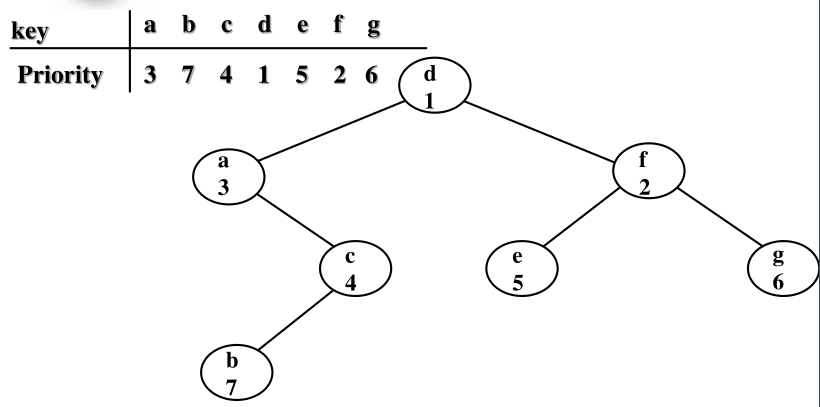
\includegraphics[width = \textwidth]{./images/treap1.png}
					\end{figure}
					Here's a little implementation of Treaps written in Ruby
					\begin{lstlisting}[language = Ruby]
class Treap
  attr_accessor :root

  def initialize(root_node)
    if root_node.is_a? TreapNode
      @root = root_node
    else
      throw "Not a valid node"
    end
  end

  # insert a value in the treap:
  # tree-insert + heap-property-restore
  def insert(value, priority)
    newNode = tree_insert(value, priority, root)
    heap_restore(newNode)
  end

  private # --------------------------------------------
 
  # binary search tree insert operation
  # right values higher
  def tree_insert(value, priority, node)
    if value > node.value
      if node.right.nil?
        node.right = TreapNode.new(value, priority)
        node.right.father = node
        return node.right
      else 
        tree_insert(value, priority, node.right)
      end
    else
      if node.left.nil?
        node.left = TreapNode.new(value, priority)
        node.left.father = node
        return node.left
      else
        tree_insert(value, priority, node.left)
      end
    end
  end

  # heap property restoring subroutine
  def heap_restore(leaf)
    if leaf != root and leaf.priority > leaf.father.priority   
      # need to rotate the tree
      if leaf == leaf.father.left
        rotate_right(leaf)
      else
        rotate_left(leaf)
      end

      heap_restore(leaf.father)
    end
  end
 end
					\end{lstlisting}
				
			\subsubsection{Skip Lists}
				Skip lists are sequential data structures (like an ordered array) that can on average maintain $O(\log(n))$ complexity for most operations. The idea is pretty simple: we add an \textit{additional pointer} to some nodes that makes you "skip" portions of the structure when followed.
				\begin{figure}[H]
					\centering
					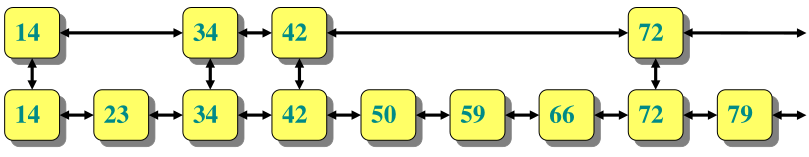
\includegraphics[width = \textwidth]{images/skipList.png}
				\end{figure}
				This creates an "overlay list" where some passages make you skip entire portions of the list, saving some accesses. The \verb|SEARCH(x)| operation starts in the fast line, then "descends" in the lower line when we're close to the \emph{x} element.\\
				The ideal skip list has half the elements per line wrt the lower line, alla evenly spaced: obviously managing such a structure during a \verb|INSERT| operation is a mess, so we can randomize something in order to statistically improve the performance of this structure:

				\paragraph{Random Skip List}
					On an insert in the bottom level, we \textit{upgrade} the element also to the upper level with a 50\% probability, and again for upper level with 50\% probability and so on; this makes 25\% the probability to be raised to the second level, 12,5\% to the third etc.\\
					This implementation of skip lists gives us a $O(\log(n))$ search complexity \underline{for all search} with high probability.

	\clearpage
	\part{Parallel Programming}
	\section{Machines and Models}
		We need a model for our machine in order to design our algorithm in a complete and coherent way, wrt the architecture they will be run on. The most used one is the RAM, or Random Access Machine

		\paragraph{Random Access Machine}
			A RAM is characterized by:
			\begin{enumerate}
				\item unbounded number of local cells
				\item unbounded cell dimension
				\item an instructions set
				\item all operation are executed in the same time
			\end{enumerate}
			These properties of the RAM define the time complexity as the number of intructions executed and the space complexity as the number of memory cells used (for an algorithm, of course).

		\subsection{Parallel Random Access Machine}
			The pretty straightforward extension to embed parallelism into a RAM is to multiply the total number of processors in it. To be more general possible, we identify each processor as a single RAM, and we add a number of input and output cells, alongside a \textit{shared memory bank of cells}.\\
			Formally, a PRAM is an \underline{unbounded collection of RAM processors}, with shared memory cells. Given that each operation (read from input, write on output read or write in memory) is done \underline{simultaneously} by all processors, we have to account for shared memory conflicts. The models of PRAM to avoid conflicts are:
			\begin{itemize}
				\item \textbf{Exclusive read}: all processors can read simoultaneously from \underline{distinct} memory location
				\item \textbf{Exclusive write}: all processors can write simoultaneously to \underline{distinct} memory location
				\item \textbf{Cuncurrent read}: all processors can read simoultaneously from \underline{all} memory location
				\item \textbf{Cuncurrent write}: all processors can write simoultaneously to \underline{all} memory location; which value "wins the race"? Priority methods can be adopted, or allowing cuncurrent writes only if the value is the same from all processors...
			\end{itemize}
			The PRAM is to parallel algorithms what the RAM is to simple algorithms: a natural abstraction of a machine that allows equal performance evaluation in a simple manner.

		\subsection{Extension of Complexity to PRAM}
			We'll extend the basic definitions to the parallel world:
			\begin{itemize}
				\item $T^*(n)$ complexity for a \underline{sequential} algorithm on a single processor
				\item $T_p(n)$ complexity on \emph{p} processors
				\item $SU_p(n) = \frac{T^*(n)}{T_p(n)}$ speedup
				\item $E_p(n) = \frac{T_1(n)}{pT_p(n)}$ efficency: work on 1 over work that can be carried out on \emph{p}
				\item $T_{\infty}$ shortest run time
				\item Cost: $P(n)\, \times\, T(n)$ 
			\end{itemize}

			\subsubsection{Matrix Vector Multiplication}
				Classic $Ax = b$ problem of multiplying matrix \emph{A} with vector \emph{x}. The problem is parallel \textit{per se}: every element in the result vector is calculated indipendently from the others. We split the computations following this concept: every processor will have to read a line of matrix \emph{A} and all vector \emph{b} and compute the polynomial value for the result.\\
				Performance evaluation:
				\begin{itemize}
					\item $T_1(N^2) = O(N^2)$
					\item $T_p(N^2) = O(\frac{N^2}{p})$ linear speedup
					\item $E_p = \frac{n^2}{p\, \times\, \frac{n^2}{p}} = 1$ perfect efficency
				\end{itemize}

			\subsubsection{Matrix Matrix Multiplication}
				Conceptually, just an extension of the previous problem to support matrix per matrix. If \emph{n} is the lenght of the matrix (suppose squared) we need $n^3$ processors\footnote{\emph{n} processors for the sum, $n^2$ total sums}. The idea is that each processor calculates the single element of the resulting matrix, so reading a row and a column of the two factors.\\
				The algorithm:
				\begin{enumerate}
					\item Read row of \emph{A} and coloumn of \emph{B} $\rightarrow$ cuncurrent read
					\item multiply elements and sum all together (using \emph{n} processors for \emph{n} elements $\rightarrow$ logarithmic cost for the sum)
					\item store values $\rightarrow$ exclusive write
				\end{enumerate}
				Performance:
				\begin{itemize}
					\item $T_1=n^3$
					\item $T_{p = n^3} = \log n$ the reduced complexity to $\log n$ is due to the possibility to use \emph{n} processors to reduce the complexity of a sum to the logarithm of its size
					\item $SU = \frac{n^3}{\log n}$
					\item $E_{n^3} = \frac{1}{\log n}$
				\end{itemize}
				graph of the performance indexes wrt the number of processors:
				\begin{figure}[H]
					\centering
					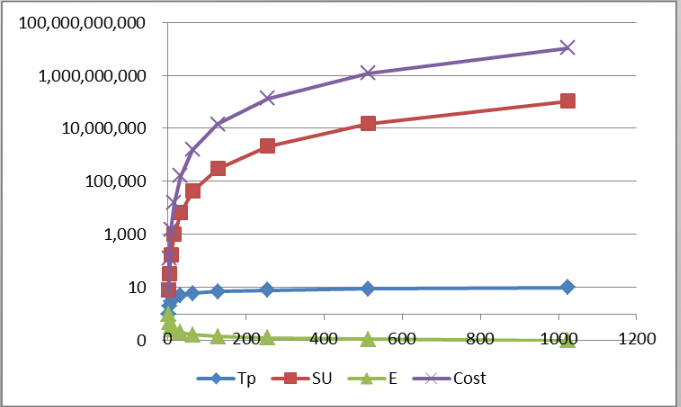
\includegraphics[width = \textwidth]{./images/perf1.png}
				\end{figure}

	\section{Amdahl's Law and Gustafson's Law}
		Amdahl's law is a mathematical formulation for calculating the speedup induced by the introduction of parallelism (multiple processors). The code is divided in \textit{serial} and \textit{parallelizable} segmentsand the speedup is calculated as
		\begin{equation}
			\begin{cases}
				f \text{ the lenght of the parallelizable part}\\
				1-f \text{ lenght of the serial part}\\
				P \text{ number of processors}\\
				SU(P, f)\, =\, \frac{T_1}{T_1*(1-f)+\frac{T_1*f}{P}}\, =\, \frac{1}{1-f+\frac{f}{P}}
			\end{cases}
		\end{equation}
		The formula is easily visualizable from
		\begin{figure}[H]
			\centering
			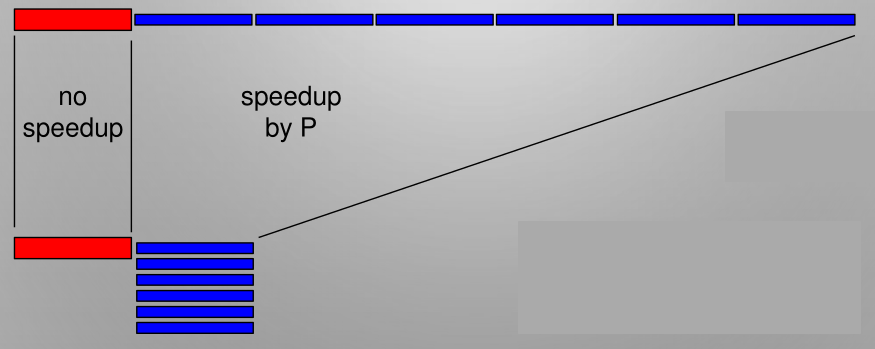
\includegraphics[width = \textwidth]{./images/Amdahl1.png}
		\end{figure}
		where the lenght of the blue part if \emph{f}.\\
		This formulation can be used to calculate the speedup upper limit wrt to the number of processors:
		\begin{equation}
			\lim_{P \rightarrow \infty} SU(P, f)\, =\, \frac{1}{1-f}
		\end{equation}
		This limit is "pessimistic": for 90\% parallelizable problems, Amdahl's law suggests to use no more than 10 processors. Gustafson's formulation "inverted" the reasoning, claiming that the parallelizable part could (more likely) not be of "fixed" lenght, while this is more likely to happen for the serial one. Se he proposed the formula
		\begin{equation}
			SU\, =\, \frac{s + P\cdot(1-s)}{s + (1-s)}\, =\, s + P\cdot(1 - s)
		\end{equation}
		where \emph{s} represents the lenght of the serial part.

	\section{Parallel Algorithms Design and Guidelines}
		Most problems have a parallel solution. Given this, designing a parallel algorithm that solves a problem is not easy task. We differenciate between
		\begin{enumerate}
			\item Parallel algorithms: the actual algorithm that solves the problem
	 		\item Parallel programs: the target specific implementation of a parallel algorithmm
		\end{enumerate}

		\subsection{PCAM Design Methodology}
			PCAM is the acronym for
			\begin{enumerate}
				\item \textbf{Partitioning}: task and data decomposition. The extremization of the "divide" part of the "divide and conquer" approach: the goal of this stage is to identify a large number of subtasks that will be executed in parallel. We take into consideration both the data and the functions:
					\begin{enumerate}
						\item Domain decomposition: the data associated to a problem is decomposed (an image into singular color layers, for example) and then the tasks working on separate data are parallelized
						\item Functional decomposition: the tasks are separated discriminating on the function they carry out, rather than the data they use. The perfect example is the model of an ecosystem: it's easier to model it by separating entities into "plants, carnivores, herbivores" etc ranther then splitting the data domain (that's also very difficult, in this case). Pipelining is a kind of functional decomposition approach.
					\end{enumerate}
					When partitioning, it's important to define "a lot"\footnote{a order of magnitude more than the processor count.} of evenly sized tasks\footnote{in order to fully exploit the parallelization}.
				\item \textbf{Communication}: task execution coordination. Tasks need to coordinate in order to achieve the computation target. The communication can be categorized with various metrics: local or global, structured or unstructured (regarding the \textit{internal organization among peers}), static ot dynamic (if the peers pool is \textit{already defined or can be discovered}), explicit or implicit (message passing or shared memory), synchronous or asynchronous, point to point or collective.\\The communication design is one of the most critical when it comes to parallel programs: it can introduce a lot of overhead (transmission and synchronization) that can even nullify the parallelization benefits. The designer should try to minimize the number of channels and try to parallelize also computation and communication.
				\item \textbf{Agglomeration}: evaluation of the structure. Clustering together tasks and combining them into larger ones is an intermediate "reduce" step. This reduces overhead because it reduces \textit{communication} and avoids a lot of \textit{data replication}. The agglomeration step is performed when we want (for example) to better exploit the locality of computation or data.
				\item \textbf{Mapping}: resource assignement. At this point, we have decomposed all the tasks, designed the communication between them, clustered some tasks. We end up with a some sort of task graph and we can start to allocate tasks to resources. Distributing tasks on a system of resource is an NP-complete problem, due to the dependency to the communication systems, the single node computational power and the single task complexity.
			\end{enumerate}
			PCAM is \underline{not} a sequential process: we may have agglomeration based on possible mappings or communication designed before partitioning.

			\paragraph{Parallel Problems are Complex}
				The main steps when writing a parallel program are 
				\begin{enumerate}
					\item Analyze the data dependencies of the problem to identify \textit{possible} parallelizations
					\item Identify hotspots, so points where most of the work is actually done. Not parallelizing hotspots can lead to bottlenecks
					\item Estimate performance against sequential solutions
					\item Repeat from 1)
				\end{enumerate}
				most of the parallelism is identified by hand, a few tools can design a tasks graph or a node network automatically.
		
		\subsection{Parallel Programming Patterns}
			\paragraph{Dependencies}
				Parallelization will always depend on the sequence of operations that are actually needed to complete a task. Those operations have \textit{dependencies} among them that constraint the order in which they're executed. We can distinguish between 3 basic dependency types:
				\begin{itemize}
					\item True dependency: \verb|a = 3; b = a;|
			 		\item Output dependency: \verb|a = function(x); a = b;|
					\item Anti dependency (pipeline problem): \verb|a = b; b = 1;|
				\end{itemize}
				\textbf{Two instructions can execute in parallel if and only if there are \textit{no depenencies} among them}.
			
			\subsubsection{Nesting Pattern}
				This is a pseudopattern: it just represents the ability to \textit{hierarchically compose} tasks, that can be themselves arranged in patterns.
				\begin{figure}[H]
					\centering
					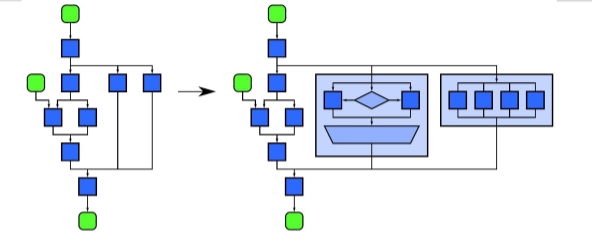
\includegraphics[width = \textwidth]{./images/Nesting.png}
				\end{figure}

			\subsubsection{Serial Control Patterns}
				All the serial programming "patterns"\footnote{more "constructs", in this case} are obviously available in the parallel framework: things as selection, iteration and sequence are still there.

			\subsubsection{Fork Join}
				This pattern focuses on the behaviour of single tasks. Forking a task means split it into two threads of execution, that may or may not be connected one another. They should rejoin later. This is the classic fork-join approach to processes in C. Joins are differnt from Barriers, as primitives: a Join requires all threads but one to terminate, while a barrier is just a sync point (all threads continue).

			\subsubsection{Map, Reduce and Filter}
				The classic functional operations can also be interpreted as parallel patterns; this is also caused by their "propention" to be parallelized: it's easy to see how a \verb|map| function can be spread among parallel tasks, or equally a \verb|filter| or a \verb|reduce| (this last one with the hypothesis that the operation of reduction is commutative and associative).

				\paragraph{Map}
					Very classic functional primitive: an operation is applied to all the elements of a collection; "do the same thing many times". The parallelization scope is huge: we can parallelize even the single elements being mapped. The strenght / weakness of the \verb|map| is that the operation is applied to \textit{the single elements}, so each iteration of the loop is \textit{indipendent from the others}. For this to be possible we need to put some constraints on the mapping function: it should be stateless (it should not depend from a shared state, or a state in general: it should be a \textit{pure} function). The map can be easily extended to multiple input collections.

			\subsubsection{Stencil, Recurrence and Scan}
				The stencil patterns is easily visualizable on a grid, that can be a grid of data or a grid of "adjacent threads". It can be seen as a \textit{generalized map}, where the function is not anymore applied to all the dataset (or threadset) but only to a selected subgroup of elements. Usually neighbours are identified by relative offsets. For the stencil pattern, boundary conditions of access must be considered, in order to avoid superpositions. \textbf{Scan} instead is a modification of the \verb|reduce| operation: a \verb|scan| applied to a collection also gives as output all the intermediate results. A parallelized scan usually needs more operations than a serial one, due to the dependencies among loop iterations.
				\begin{figure}[H]
					\centering
					\begin{subfigure}{0.5\textwidth}
						\centering
						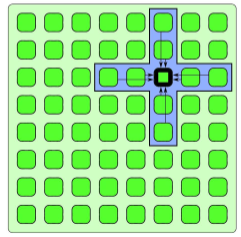
\includegraphics[width = 0.4\linewidth]{./images/Stencil.png}
					\end{subfigure}%
					\begin{subfigure}{0.5\textwidth}
						\centering
						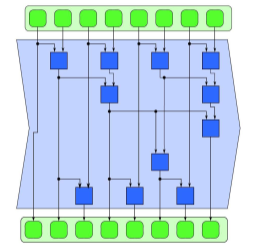
\includegraphics[width = 0.4\linewidth]{./images/Scan.png}
					\end{subfigure}
					\caption{Stencil and Scan operation}
				\end{figure}
				The recurrence operation instead is a complex version of the \verb|map|, where single elements can be passed through the mapping function \textit{alongside adjacent ones}. For a recurrence to be computable, there \textit{must} be a serial ordering of the recurrence elements. A recurrence can also be seen as a stencil where neighbours are accessed \textit{both as inputs and outputs}: a one-dimensional recurrence is a \verb|scan|, in fact.

				\paragraph{Stencil}
					Stencil is, as said, a supermap operation that keeps into account neighbouring data when computing a function on a dataset. So for example, viewing an image as a matrix of pixels, a "smoothing" function is perfectly applied through a stencil-like operation that averages color intensity around certain points.

		\subsection{Parallel Data Management Patterns}
			Parallel programs deals with data in various ways. The management of the memory varies according to how data is read, written, shared, allocated and copied.
			\begin{enumerate}
				\item \underline{Random read and write} policy explains itself: memory locations are managed through pointers, that represents addresses. Aliasing (superposing of memory location) can be a problem.
				\item \underline{Stack allocation}: dynamically allocate data in a LIFO manner. In a parallelized world, each thread of execution receives his own stack; this way thread locality is preserved.
				\item \underline{Heap allocation} is the opposite of stack allocation; again different memory section/pools are to be kept for each thread. Queue allocation strategies are also more complex and and slower to implement wrt stack ones.
				\item \underline{Objects}: we can also manage the memories in a OO way, trying to bundle together data and data transformations. This varies significatively among parallel programming models.
			\end{enumerate}
			We can give also a firther characterization of parallel data management patterns:

			\subsubsection{Pack}
				Pack is the process of reducing a collection by removing the empty nodes. Usually it's implemented through a flagging procedure, that sweeps the collection to find idle/empty nodes. The remaining ones are then transferred in an other reduced structure. It does have a reverse \verb|unpack| primitive.

			\subsubsection{Pipeline}
				Intended as software pipeline, this is the classic approach to exploit a line of work in a consumer - producer fashion. Each node takes data from the previous one and passes elaborated data to the next; each node can so work in parallel with the others. The pipeline is usually linear, but DAG pipelines can be also built (maximizing parallelism).

			\subsubsection{Geometric Decomposition}
				Again in the data-as-matrix realm. We can divide our pool of data in sections (that can be overlapping also) and assign them to tasks. It's a tetris game.
				\begin{figure}[H]					
					\centering
					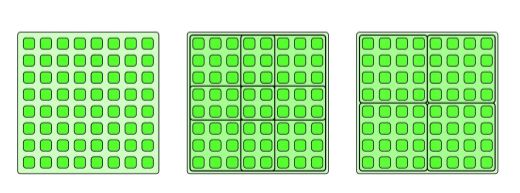
\includegraphics[width = \textwidth]{./images/GDec.png}
				\end{figure}
				This pattern does not necessarily move data, it just groups together nodes.\\
				We can classify decomposition with two criteria: if data is overlapping or not, and if pertitions are homogeneous or not. The resulting schema is\\
				\begin{tabular}{c || c | c }
					& Overlapping Partitions & Non overlapping partitions\\
					\hline
					\hline
					Uniform partitions & \textit{decomposition} & \textit{partitioning}\\
					Non uniform partitions & \textit{decomposition} & \textit{segmentation}					
				\end{tabular}

			\subsubsection{Gather and Scatter}
				Gather and Scatter are two opposite patterns: they both require a data collection and a set of indices (or locations) as input and output a new reordered and filtered set, but the use of the auxiliary index collection is different; gather \textit{reads elements accessing the input collection using the index collection as a mask}, so also ordering the input collection as specified in the index (indexes can be non-unique). The scatter is the opposite: the indexes collection is used during the \verb|write operation|, instead of in the \verb|read| one.
				\begin{lstlisting}[language = c]
void scatter(int *input, int *indexes, int *output){
	for(int i = 0; i < BUFFERSIZE; i++)
		*(output + *(indexes + i)) = *(input + i);
}

void gather(int *input, int *indexes, int *output){
	for(int i = 0; i < BUFFERSIZE; i++)
		*(output + i) = *(input + *(indexes + i));
}
				\end{lstlisting}
				Gather has several special cases (that are just more trivial) that can offer more parallelization possibilities. One is the \verb|shift|, the classical "move all elements of an array by n positions left or right". A parallel implementation can rely on \textit{vector intrsuctions} in order to move all data at a time\footnote{Given that the boundary elements, that need to be shifted in/out from the collections, are handled properly.}. Another particulare case is the \verb|zip| pattern, where two collections are interleaved (and so merged) into a last collection. Obviously there exists a \verb|unzip| pattern.\\
				Scatter has a writing problem: what happens if write positions are duplicated, so if multiple value must be written in the same place? There are several solutions:
				\begin{enumerate}
					\item \underline{permutation scatter} that checks whether in the indxes array aren't present duplicates
					\item \underline{atomic scatter} which non-deterministically solves conflicts (keeping operations atomicity)
					\item \underline{priority scatter} that solves conflicts by adding a priority to each element
					\item \underline{merge scatter} that instead solves conflict by merging together the conflicting elements (in numbers, summing them for example).
				\end{enumerate}

				\paragraph{Converting Scatter to Gather}
					Scatter is more expensive than gather; this is true for a number of reasons: writing is generally more expensive than reading (cache may block micro-writes) and all cores should synchronize to maintain cache coherency. All the cache\footnote{and architecture} related problems can be fully avoided if we know in advance which addresses (indexes) will be used. In fact, all forms of scatters can be transformed into gathers if the indexes are known in advance.
				
	\section{Dynamic Programming}
		Dynamic programming is a technique to solve problems that resembles divide and conquer: it partitions the problem into smaller subproblems then merges the results. It's applicable when two properties are verified:
		\begin{itemize}
			\item Optimal substructure
			\item Overlapping subproblems
		\end{itemize}

		\paragraph{Optimal Substructure}
			A problem is said to have an optimal substructure when an optimal solution can be built directly from the solutions of its subproblems. More in concrete, an optimal solution of the problem can be found \textit{among the optimal solutions of the subproblems}\footnote{as the branch and bound methods.}. 
		
		\paragraph{Overlapping Subproblems}
			We say that a problem has overlapping subprolems if the problem can be splitted in several subproblems \textit{which are reused many times}. The classic interpretation / visualization of this property is a decision binary tree where there are "twin subtrees" - subtrees with the same identical structure and node values.\\
			A "splitting" algorithm \textit{without} the overlapping subproblems property is a classic divide and conquer algorithm.

		\paragraph{Intermediate Results Memoization}
			A dynamic programming approach aims to avoid the \textit{recomputation} of intermediate results, the ones that come from the overlapping subproblems. Instead, these results are stored and accessed when needed (avoiding so to re-execute the entire computation.

		\subsection{Longest Subsequence Example}
			\textbf{The problem}: given two symbols ordered collections, find a longest subsequence common to them both, even not consecutive symbols. For example, collections \verb|a c a d a f a r t| and \verb|a b c| share the \verb|a c| subsequence.\\
			\textbf{The approach}: we focus first on finding the \textit{length} of the LCS, then we extend the algorithm to find the exact sequence\footnote{we use this approach because I said so.}.\\
			\textbf{The algorithm}: easy enough: the most basic formulation scans all the second vector elements \textit{for each element in the first one}, to compare the values. The divide and conquer recursive approach works in a similar way: we analyze the couple of elements in the current index, and if they're equal we decrease \underline{both} indexes, if not we recusively call two times the procedure (one for the index we're decrementing). The pseudocode\footnote{I hate it too, but it's the fastest way trust me} is
			\begin{figure}[H]
				\centering
				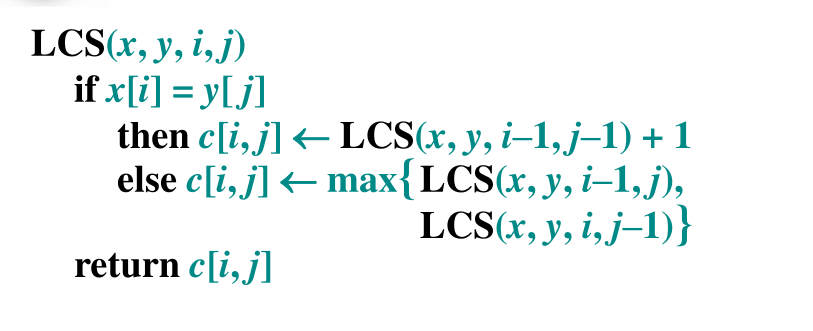
\includegraphics[width = \textwidth]{./images/LCS.png}
			\end{figure}
			Where \verb|x, y, i, j| represents the two vectors and the two indexes, respectively. This approach is obviously similar to a DaC one; however, we can easily identify a set of problems that both recursive calls will go through:
			\begin{figure}[H]
				\centering
				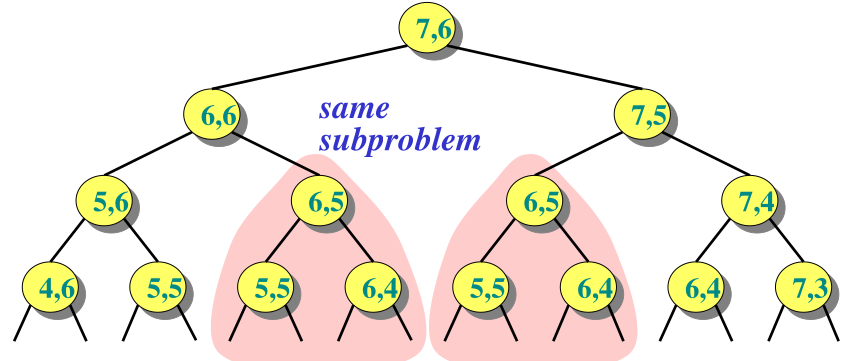
\includegraphics[width = \textwidth]{./images/LCStree.png}
			\end{figure}
			So, we should now find a way to buffer the already computed elements. Easy enough to do, we build a matrix that's $\vert x \vert \times \vert y \vert$ big, and store there the results of the computation. Prior to evaluate a certain intermediate result, we check the matrix for it. Memoized version of the algorithm:
			\begin{figure}[H]
				\centering
				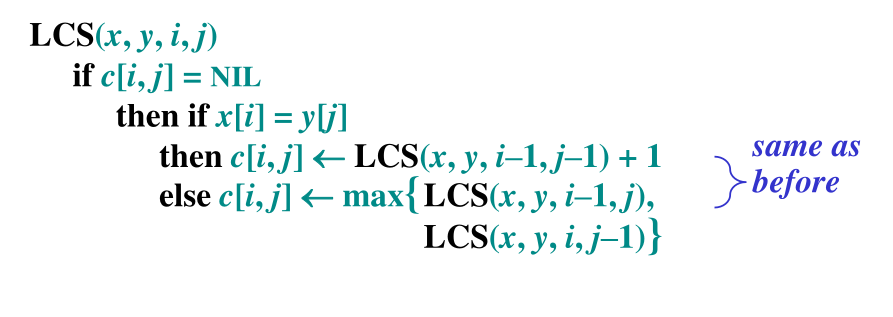
\includegraphics[width = \textwidth]{./images/MLCS.png}
			\end{figure}
	
	\section{Amortized Analysis}
		Amortized analysis is a technique used to compute the time needed to perform a certain set of operations; it averages the time required to do an operation over all the operations performed. The goal is to show that an operation is small when compared to the whole set of operations, even though a single operation can be expensive.\\
		\textbf{Amortized analysis is not average-case analysis}: probability is not involved here, and this method \textit{guarantees the average performance of each operation} in the worst case. It's an alternative to worst-case analysis to compute the running time of an algorithm.

		\paragraph{Aggregate analysis}
			We analyze the problem of adjusting the size of an hash table in order to keep it as small as possible \textit{and} not having overflow lists. The first idea is to reallocate the whole table whenever an overflow is detected, with the total space doubled. This way, the insertion of a single element will have constant complexity unless exactly $2^n-1$ elements have been inserted, in that case the cost will be equal to $2^n$ (n being the size of the table).\\
			If we analyze the complexity in the classic worst-case approach, we see that since a single insertion can cause the re-insertion of all the previous elements (due to the reallocating in case of overflow) the overall complexity is $\Theta(n^2)$.
			\begin{figure}[H]
				\centering
				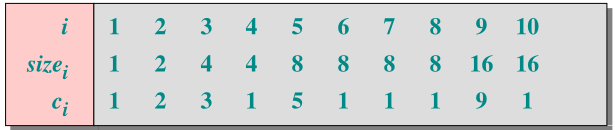
\includegraphics[width = \textwidth]{images/amortized1.png}
			\end{figure}
			\begin{figure}[H]
				\centering
				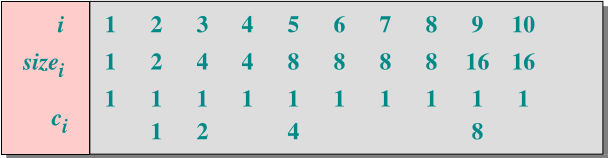
\includegraphics[width = \textwidth]{images/amortized2.png}
			\end{figure}
			Where \emph{i} is the element inserted, $c_i$ the overall cost of inserting the element and $size_i$ the current size of the table.\\
			The cost for n insertions then become:
			\begin{equation}
				\sum_{i=1}^{n}(c_i)\, \leq\, n\, +\, \sum_{j=0}^{\lfloor \log(n-1) \rfloor}(2^j)\, \leq\, \underbrace{3n}_{2^{\log(n)}\, \approx\, n}\, =\, \Theta(n)
			\end{equation}

		\subsection{Accounting method}
			The accounting method aims to be more precise of the aggregate one, by using helper values and variables in the analysis.\\
			We associate to every operation a fictitious cost $\hat{c}$ and we then compute the total complexity with that cost. Any amount not consumed is accumulated in a "bank"; out goal is to have in the "bank" a non negative value, so we can be sure to have provided an upper bound to the complexity of the algorithm.\\
			For the hash table dynamic size problem, we can set a cost of 3 for each operation:
			\begin{itemize}
				\item 1 is the cost of the insertion
				\item 2 is the cost of doubling the size
			\end{itemize}
			So if we analyze the sequential insertion of elements in the hash, as we've done before, we increment our "bank" value each step by the difference of the amortized cost and the real one:
			\begin{figure}[H]
				\centering
				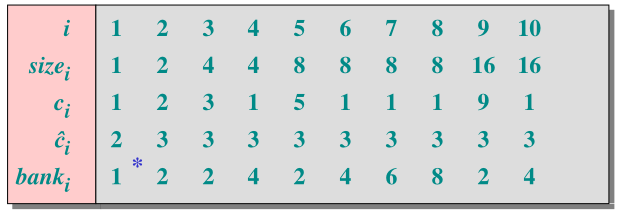
\includegraphics[width = \textwidth]{images/accounting1.png}
				\caption{We can see how the "bank" value never goes negative, so the sum of the amortized costs provides an upper bound on the sum of true cost}
			\end{figure}

		\subsection{Potential method}
			As the accounting method, the potential one accumulates cost "on the go" and tries to compute the cost by expressing it as a recursive formula (a-la dynamic programming).\\
			In detail: we have our $D$ data structure, and operation $i$ transforms $D_{i - 1}$ to $D_i$ at cots $c_i$. We also need a potential function defined as
			\begin{equation}
				f:\, \{D_i\}\, \rightarrow\, R^+
			\end{equation}
			That assigns at each state a non negative real number for each step. We can now define the amortized cost at step \emph{i} as
			\begin{equation}
				\hat{c}_i \,=\, c_i + \underbrace{f(D_i) - f(D_{i-1})}_{\text{potential difference}\, \Delta f}
			\end{equation}
			The reasoning is pretty much the same as in the accounting approach: if the $\Delta f$ is positive at step $i$, then cost is being accummulated in the data structure; otherwise, the cost accumulated is being used to compensate a very expensive operation. If we put all together
			\begin{equation}
				\sum_{i = 1}^n\hat{c}_i \,=\, \sum_{i = 1}^n(c_i + f(D_i) - f(D_{i - 1})) \,=\, \underbrace{\sum_{i = 1}^nc_i + f(D_n) - f(D_0)}_{\text{the series telescopes}}
			\end{equation}
			So the total amortized cost is bigger than the sum of all standard costs, because the cost of the final state is greater than zero but $f(D_0) = 0$\footnote{property of $f(x)$}
	
	\section{Competitive Analysis}
		Competitive analysis is a method that aims to provide a measure of the complexity of an \textit{online algorithm} by comparing it the equivalent \textit{offline version}. This is usually done when probabilistic estimations on the input are not available (so most of the cases).\\
		The comparison is done looking at the worst case complexity if the online algorithm we're analyzing versus the worst case complexity of the best offline algorithm available, also called God's algorithm (differently from the online one, n fact, it knows all future inputs that will come). An algorithm is said to be alpha competitive is it's only linearly more complex (additive constants exluded) wrt the optimal offline version, or more formally
		\begin{equation}
			C_{online}(S) \,\leq\, \alpha \cdot C_{offline optimal}(S) + k
		\end{equation}
		where $S$ represents the sequence of operations taken into consideration.

		\paragraph{Self Organizing Lists}
			Say we wanto to implement a linked list, and we want to make so that the implementation can adapt to the requests in order to speedup the accessing of elements. This will not change the worst case complexity (it will remain $O(n)$ of course) but could significatively improve the average seek time. We have to introduce heuristics to do so:
			\begin{itemize}
				\item \textbf{Move to front}: this heuristic simply takes the accessed element and moves it at the first place of the list. Since moving an item of n positions (that we will call \textit{rank}) costs n, we have that the total cost of finding + reordering is
					\begin{equation}
						c \,=\, 2 \,\cdot\, rank(x)
					\end{equation}
					where $x$ is the accessed element. This heuristic is $\alpha$ competitive for self organizing lists, more precisely 4-competitive. Let's try to prove it:\\
					We use as potential function
					\begin{equation}
						\Phi(L_i) \,=\, 2 \,\cdot\, \text{number of inversions}
					\end{equation}
					where the number of inversions is formally defined as a function on couples
					\begin{equation}
						\text{number of inversions} \,=\, |(x, y) \,:\, x \prec_{L_i} y \,\wedge\, y \prec_{L_i^*} x |
					\end{equation}
					where $\prec_{List}$ stands for "precedes in list $List$". An access to an element brings it to the front, so moving all preceding elements before him a "step forward", causing the destruction / creation of some other inversions REMEMBER: WITH INVERSIONS WE ARE COMPARING IT TO THE OPTIMAL LIST WITH THE OPTIMAL ALGORITHM.\\
					To prove the $\alpha$-competitivity, we consider each element of lists $L$ and $L^*$ which are respectively the one with the online MTF algorithm and the offline optimal. We can categorize each element of the lists basing ourselves on the inversions it is part of, wrt a $x$ element tha would be the searched one:
					\begin{itemize}
						\item precedes $x$ in both lists
						\item precedes $x$ in $L$ and follows $x$ in $L^*$
						\item follows $x$ in $L$ but precedes $x$ in $L^*$
						\item precedes $x$ in both lists
					\end{itemize}
					more formally:
					\begin{figure}[H]
						\centering
						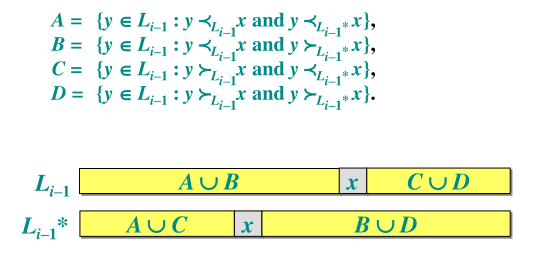
\includegraphics[width = \textwidth]{./images/MTF1.png}
					\end{figure}
					So MTF moves $x$ to the front we have two costs defined for each list as:
					\begin{equation}
						\begin{cases}
							r = |A| \,+\, |B| + 1 = \text{rank}_{L_{i - 1}}(x)\\
							r^* = |A| \,+\, |C| + 1 = \text{rank}_{L_{i - 1}^*}(x)
						\end{cases}
					\end{equation}
					so, we have
					\begin{equation}
						\Phi(L_i) - \Phi(L_{i-1}) \leq 2 \,\cdot\, (|A| - |B| + t_i)
					\end{equation}
					where $t_i$ is the number of transposes $x$ has undergone in $L^*$. If we make the amortized cost calculation now:
					\begin{align}
						\hat{c}_i = c_i + \Phi(L_i) - \Phi(L_{i - 1})\\
						\leq 2r + 2(|A| - |B| + t_i)\\
						= 2r + 2(|A| - (r - 1 -|A|) + t_i)\\
						= 4|A| + 2 + 2t_i \leq 4(r^* + t_i) = 4c_i^*
					\end{align}
					So obtaining that the amortized cost is linearly dependent from the optimal cost.
				\item \textbf{Count method}: alongside each element store a count of the times it has been accessed and keep the list reversely ordinated according to that count
				\item \textbf{Transpose/bubble method}: each time a node is accessed, it's swapped with the preceding node
			\end{itemize}

	
	\clearpage
	\section{Implementations}
		\subsection{Posix PThreads}
			Posix threads are an implementations of a shared memory parallel programming model based on threads. In UNIX systems, a thread is a "subprocess" in the sense that is a process' son, but it's indipendent from the process execution or the execution of other "brothers" threads. Multi threading software architecture are thus lighter than just multi process ones, because threads, when spawned, needs to duplicate the bare minimum amount of data; in fact, they share most of the father process information.\\
			PThreads makes use of \textit{explicit synchronization} through primitives and \textit{implicit communication} through shared variables, usually accessed through pointers. This model of communication is prone to \textit{data race conditions}, where more threads competes for a resource access (the accesses are cuncurrent).

			\subsubsection{Synchronization Primitives}
				The PTrhead standard has several synchronization primitives to use:
				\begin{itemize}
					\item \verb|join|: a thread calling \verb|join| \textit{stops and waits for all his sons to complete}. A thread, if joinable, can become \textbf{detached} so doea not have a father thread.
					\item \verb|barrier|: a barries is like a \verb|join| but the threads do not terminate on the synch. It's just a "numbered checkpoint" that aligns all the threads executions. Super useful when defining software pipelines.
					\item \verb|mutex|: not exactly a synchronization primitive \textit{per se}, as it's used only to access shared resources.
					\item condition variables: created through the \verb|pthread_cond_wait| primitive, they're just enhanced mutexes. They allow threads to synchronize explicitly. They avoid polling continously the mutex to see if it's locked.
				\end{itemize}

				\paragraph{Barriers Join Example}
					As a first "Hello World" example, we're trying to have two threads snchronize to print a message in a serial way. Notice how the barrier is used, and how the main thread has to wait for the last to terminate. Why this? Because if not, it can happen that the main thread terminates before his sons, having them to abrutly end mid-execution.
					\begin{lstlisting}[language = c]
#include <pthread.h>
#include <stdio.h>
#include <stdlib.h>

typedef struct {
   int index;
   pthread_barrier_t *sync;
} thread_param_t;

pthread_barrier_t barrier;

void * thread_body(void *param){
   int local_index = ((thread_param_t *)param)->index;
   if(local_index == 1){
      printf("  Thread 1 speaking: FIRST\n");
      pthread_barrier_wait(((thread_param_t *)param)->sync);
   } else {
      pthread_barrier_wait(((thread_param_t *)param)->sync);
      printf("  Thread 2 speaking: LANDING\n");
   }
}

int main(int argc, char * argv){
   // sync barrier init
   pthread_barrier_init(&barrier, NULL, 2);

   thread_param_t *pt1 = malloc(sizeof(thread_param_t)),
                  *pt2 = malloc(sizeof(thread_param_t));

   pt1->index = 1;
   pt1->sync = &barrier;

   pt2->index = 2;
   pt2->sync = &barrier;

   // thread pool
   pthread_t threads[2];

   printf("Starting threads:\n");

   // thread initialization
   pthread_create(&threads[0], NULL, thread_body, (void *)pt1);
   pthread_create(&threads[1], NULL, thread_body, (void *)pt2);

   // wait for last thread to end
   pthread_join(threads[1], NULL);
   printf("exiting...\n");

   return 0;
}
					\end{lstlisting}
				

				
\end{document}

